\documentclass[12pt, a4paper]{report}
\usepackage[utf8]{inputenc}
\newcommand\preamble{
    \usepackage[italian]{babel}
    \usepackage{geometry}
    \usepackage{amsmath}
    \usepackage{amssymb}
    \usepackage{graphicx}
    \usepackage{ulem}
    \usepackage[table, dvipsnames]{xcolor}
    \usepackage{tikz}
    \usepackage{qtree}
    \usepackage{spverbatim}
    \usepackage{hyperref}

    \geometry{margin=2cm}
    \let\olditemize\itemize
    \renewcommand\itemize{\olditemize\setlength\itemsep{0em}}
    \graphicspath{{Immagini/}}

    \author{Lorenzo Vaccarecci}

    \hypersetup{
        colorlinks=true,
        linkcolor=blue,
        filecolor=magenta,      
        urlcolor=blue,
        pdfpagemode=FullScreen,
    }

    \urlstyle{same}
}
\newcommand{\red}[1]{\textcolor{red}{#1}}
\preamble

\begin{document}
\begin{titlepage}
    \centering
    \vfill
    {\bfseries\Huge
        Appunti Analisi e Progettazione Algoritmi\\
        \vskip1cm
        \Large
        Lorenzo Vaccarecci\\
        \vskip1cm
        \normalsize
        A.A. 2023/2024
    }
    \vfill
    \vfill
    \vfill
\end{titlepage}
\tableofcontents
\chapter{Analisi della correttezza e complessità degli algoritmi}
\section{Notazioni asintotiche}
\begin{itemize}
    \item Una funzione $f(n)$ appartiene all'insieme $O(g(n))$ se da un certo punto $n_{0}$ in poi, $f$ sta sotto una funzione "multipla" di $g$ \begin{center}
        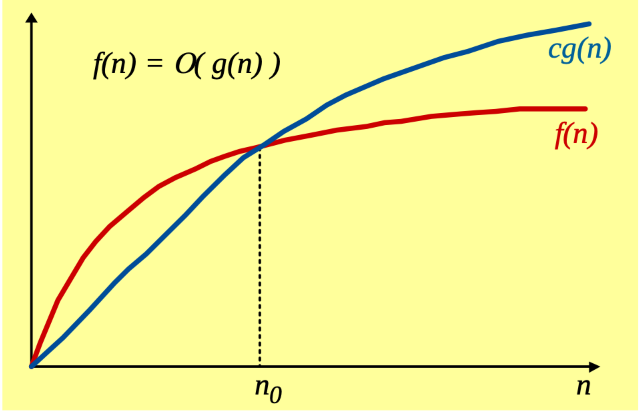
\includegraphics[scale=0.5]{bigO.png}
    \end{center}
    \item Una funzione $f(n)$ appartiene all'insieme $\Omega(g(n))$ se da un certo punto $n_{0}$ in poi, $f$ sta sopra una funzione "sottomultipla" di $g$ \begin{center}
        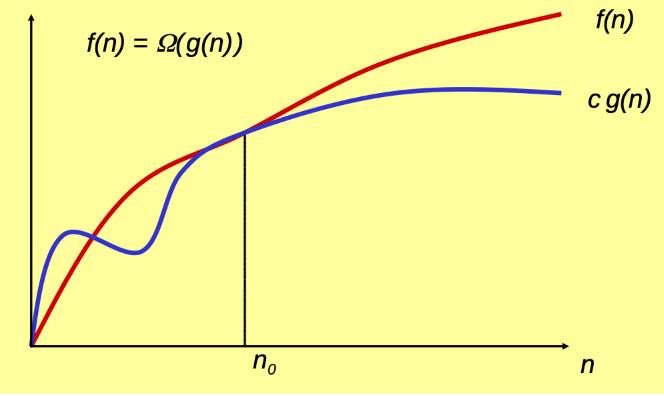
\includegraphics[scale=0.5]{Omega.png}
    \end{center}
    \item Una funzione $f(n)$ appartiene all'insieme $\Theta(g(n))$ se da un certo punto $n_{0}$ in poi, $f$ è compresa tra un "multiplo" di $g$ e un sottomultiplo di $g$ \begin{center}
        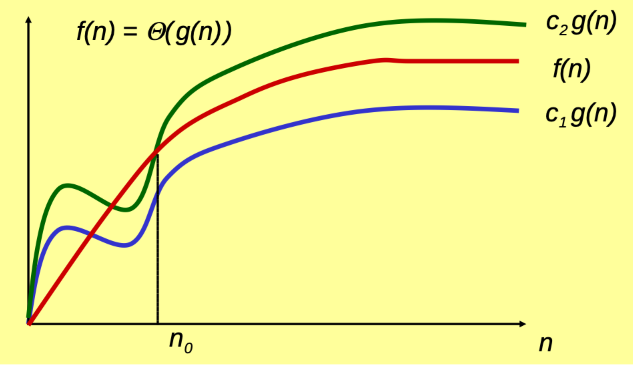
\includegraphics[scale=0.5]{Theta.png}
    \end{center}
\end{itemize}
\subsection{Proprietà della notazione asintotica}
\subsubsection{Transitiva}
\begin{itemize}
    \item $f(n)$ è $O(g(n))$ e $g(n)$ è $O(h(n))$ implica $f(n)$ è $O(h(n))$
    \item $f(n)$ è $\Omega(g(n))$ e $g(n)$ è $\Omega(h(n))$ implica $f(n)$ è $\Omega(h(n))$
    \item $f(n)$ è $\Theta(g(n))$ e $g(n)$ è $\Theta(h(n))$ implica $f(n)$ è $\Theta(h(n))$
\end{itemize}
\subsubsection{Riflessiva}
\begin{itemize}
    \item $f(n)$ è $O(f(n))$
    \item $f(n)$ è $\Omega(f(n))$
    \item $f(n)$ è $\Theta(f(n))$
\end{itemize}
\subsubsection{Simmetrica}
$f(n)$ è $\Theta(g(n))$ se e solo se $g(n)$ è $\Theta(f(n))$
\subsubsection{Simmetrica trasposta}
$f(n)$ è $O(g(n))$ se e solo se $g(n)$ è $O(f(n))$
\subsubsection{Somma}
$f(n)+g(n)$ è $O(\max\{f(n),g(n)\})$, analogamente per $\Omega$ e $\Theta$
\subsubsection{Comportamenti notevoli intrattabili}
\begin{itemize}
    \item $\Theta(2^{n})$ esponenziale
    \item $\Theta(n!)$ fattoriale
    \item $\Theta(n^{n})$ esponenziale in base $n$
\end{itemize}
\newpage
\section{Complessità di algoritmi e problemi}
\textbf{Legenda:}
\begin{itemize}
    \item $n$: dimensione dell'input
    \item $i$: un input
    \item $t(i)$: tempo di esecuzione dell'algoritmo per l'input i
    \item $s(i)$: spazio di memoria necessario per l'esecuzione dell'algoritmo per l'input i
\end{itemize}
\textbf{Complessità temporale}
\begin{itemize}
    \item \textbf{Caso peggiore} $T_{worst}(n)=\max\{t(i)|i \text{ ha dimensione } n\}$
    \item \textbf{Caso migliore} $T_{best}(n)=\min\{t(i)|i \text{ ha dimensione } n\}$
    \item \textbf{Caso medio} $T_{avg}(n)=\text{avg}\{t(i)|i \text{ ha dimensione } n\}$
\end{itemize}
Per il caso medio, per ogni $n$ si considerano tutti i possibili input di dimensione $n$, siano $i_{1},\ldots,i_{N}$ e si fa la media aritmetica dei tempi:\\
$T_{avg}(n)=\frac{t(i_{1})+\ldots+t(i_{N})}{N}$\\
Ovviamente, se i possibili casi di input non sono equiprobabili la media deve essere una media pesata:\\
$T_{avg}(n)=p_{1}\cdot t(i_{1})+\ldots+p_{N}\cdot t(i_{N})$\\
Definizioni:
\begin{itemize}
    \item Un algoritmo ha complessità $O(f(n))$ se $T_{worst}(n)=O(f(n))$
    \item Un algoritmo ha complessità $\Omega(f(n))$ se $T_{best}(n)=\Omega(f(n))$
    \item Un algoritmo ha complessità $\Theta(f(n))$ se ha complessità $O(f(n))$ e $\Omega(f(n))$
\end{itemize}
Per gli algoritmi randomizzati il caso peggiore è definito come:\\
$T_{exp}(i)=\mathbb{E}[t(i,c)]$ \textcolor{red}{Da completare la spiegazione di questa parte} \\
$T_{exp\_worst}(n)=\max(T_{exp}(i)|i \text{ ha dimensione } n)$\\
\textbf{\red{Problema $\neq$ Algoritmo}}
\begin{itemize}
    \item \textbf{Delimitazione superiore}: Un problema ha complessità $O(f(n))$ se esiste un algoritmo di complessità $O(f(n))$ che lo risolve
    \item \textbf{Delimitazione inferiore}: Un problema ha complessità $\Omega(f(n))$ se tutti i possibili algoritmi risolventi hanno complessità $\Omega(f(n))$
\end{itemize}
Quindi per trovare una delimitazione superiore è sufficiente (e necessario) trovare un algoritmo che risolva il problema in un tempo $O(f(n))$, mentre, per trovare una delimitazione inferiore è necessario dimostrare che qualunque possibile algoritmo deve impiegare un tempo $\Omega(f(n))$. \textbf{Un problema è \underline{chiuso} se si conoscono limite superiore e inferiore coincidenti}:
\begin{itemize}
    \item Esiste un algoritmo risolvente di complessità $O(f(n))$
    \item Si è dimostrato che qualunque algoritmo risolvente deve avere complessità $\Omega(f(n))$, ossia non può esistere un algoritmo di complessità inferiore a $\Omega(f(n))$
\end{itemize}
Si è quindi dimostrato che l'algoritmo risolvente è \underline{ottimo}. \textbf{Un problema è \underline{aperto} se (tutte le) delimitazioni inferiori e superiori differiscono} e di conseguenza ha un gap algoritmo. Un gap algoritmo può essere chiuso in due modi:
\begin{itemize}
    \item \textbf{Dal di sopra}: si trova un algoritmo migliore, abbassando così il limite superiore
    \item \textbf{Dal di sotto}: si riesce a dimostrare un limite inferiore più alto
\end{itemize}
I due modi non sono mutuamente esclusivi, ossia può succedere che si riesca a trovare un algoritmo migliore, e contemporanemante si riesca a dimostrare un limite inferiore più alto.
\section{Corretteza di algoritmi ricorsivi}
E' basata sul principio di induzione.\\
Un insieme definito induttivamente è un insieme i cui elementi sono tutti e soli quelli che si ottengono applicando ripetutamente un insieme di regole, a partire da quelle con premessa vuota che costituiscono la base della definizione induttiva.
\subsection*{Esempio: Serie geometrica}
Proviamo per induzione aritmetica che $P(n)=\sum_{i=0}^{n}q^{i}=\frac{q^{n+1}-1}{q-1}$, per tutti gli $n\in \mathbb{N}$.\\
\textbf{Base} $P(0)=q^{0}=1=\frac{q^{1}-1}{q-1}$\\
\textbf{Passo induttivo} Assumiamo $P(n)$ e dimostriamo $P(n+1)$:
\begin{equation*}
    P(n+1)=\sum_{i=0}^{n+1}q^{i}\rightarrow q^{0}+\ldots+q^{n}+q^{n+1}\rightarrow\left(\sum_{i=0}^{n}q^{i}\right)+q^{n+1}
\end{equation*}
Svolgendo i calcoli si riesce a determinare che viene
\begin{equation*}
    \frac{q^{(n+1)+1}-1}{q-1}
\end{equation*}
\end{document}